\documentclass[titlepage]{report}

\usepackage[toc,page]{appendix}
\usepackage{glossaries}
\usepackage{makeidx}
\usepackage{biblatex}
\usepackage{graphicx}
\usepackage{float}

\makeglossaries{}
\loadglsentries{entries}

\makeindex
\addbibresource{bib.bib}

\title{blockchain\_message: A Peer-to-Peer Content-Sharing Service Built on the Ethereum Blockchain\\\large System Requirements Specification}
\author{Sean T. Batzel\\Dr.\ Bishop}
\date{\today\endgraf\bigskip Submitted in partial fulfillment of the requirements of CMPS/IT 490 --- Computer Projects}

\begin{document}
\maketitle

\tableofcontents

\nocite{*}

\section{Introduction}
A major point of concern in computing in general recently has been privacy. What are companies doing with our data to leverage us as assets? If I send an email or a text message, or even make a phone call, who is privy to what's said in those communications? Can we conclusively trust the services we use? blockchain\_message is a platform which utilizes the new and growing blockchain model through Ethereum, along with time-tested encryption processes to allow for the transmission of information securely and directly, using a decentralized network to process the messages rather than a single entity. Using Ethereum, the system is designed to make messages as difficult to intercept, modify, delete, or otherwise disrupt as possible, working to make your communications as secure as they can be.

\pagebreak
\section{System Model}
\begin{figure}[H]
\centering
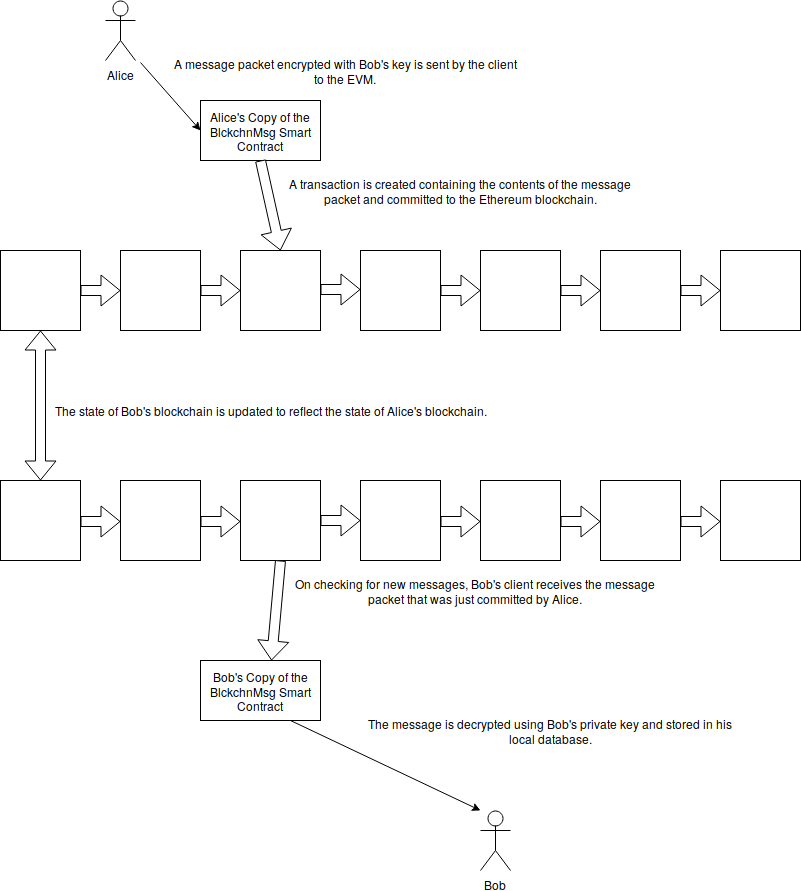
\includegraphics[width=1.3\textwidth]{diagram}
\caption{A high-level overview of blockchain\_message's functionality.}
\end{figure}
\pagebreak

\section{Functional Requirements}
\subsection{General Features Overview}
The base functionality of the application is a simple instant messaging system where messages are exchanged directly through \gls{Ethereum}\index{Ethereum} and not through a central server. Messages are encrypted and sent to a program running on the Ethereum computer, which records them in a permament and unchangeable chain to be downloaded and decrypted by the intended recipient. Ideally, users of this platform would be able to create an account for a single device that would remain completely secure for every communication sent from it.

\subsection{Security and Privacy}
The major benefit to this system being built on Ethereum\index{Ethereum} is that every message sent is recorded permanently in a transaction\index{transaction} on the blockchain\index{blockchain} in a manner that, because of Ethereum's architecture, cannot be changed. Because fairly strong RSA keypairs are used for encryption/decryption purposes, the messages are committed in such a way that it becomes prohibitively challenging to hijack them, whether to read them or to modify them. If used correctly, the system will create a new keypair for every device (assuming that the same identity is not used on multiple devices), reducing the risk that decryption keys may be stolen. Data is encrypted and committed to the blockchain on the local machine, reducing the risk that unencrypted data may be intercepted during communication. This also removes the privacy concerns for services using the standard server/client architecture, since the data is stored on every node running Ethereum there are no concerns for losing access to one's personal data.

\section{User Interface Specification}
The UI will have three levels during development, starting with a command-line interface, with a median goal being an HTML5-based graphical interface and the ultimate goal being a native Android application.

\subsection{Command-Line Interface}
The CLI will accept a few simple commands for interacting with the blockchain\_message system. On running the program, you will be met by a login screen to prompt for a user address, a username, and an email address. These three elements will be used to identify you to the network while exchanging messages.
The interface commands are as follows:

\texttt{write} - Composes and sends a new message.

\texttt{check} - Downloads any new messages and reports how many were retrieved.

\texttt{read} - Lists the text of all messages retrieved from the blockchain.

\texttt{new-contact} - Creates a new contact by prompting for a user address, a username, and an email address.

\texttt{exit} - Ends the program.

\subsection{HTML5 Interface}
As a medium-term stretch goal, I plan on implementing a simple graphical interface running locally for end users who are less comfortable with CLI operations. The HTML5-based interface will expose all of the same functionality as the command-line interface.

\subsection{Android Application}
My extreme-term stretch goal is to develop and Android application that leverages the light client specification to run the entire application locally to an Android device. The app itself will consist of a standard navigation menu with a screen for contact management (add/delete/edit/detail functions will also be exposed), a screen for message management (with the standard functionality expected from a messaging client), and a screen for profile management which will allow sharing profile information and public encryption keys.

\section{Non-functional Requirements}
\subsection{Software Requirements}
The first version of the blockchain\_message command-line interface is designed to run on Ubuntu Linux\index{Linux}, but with tweaking can be made to run on any system with Python installed. The installation script can be easily modified for installation on any Linux distribution.

The system requires that an Ethereum\index{Ethereum} \gls{node}\index{node} be accessible, which can be either set up on the local machine through Parity or Geth or exposed through a service such as Infura.io. A long-term goal is to leverage the light client specification to create a version that requires less heavy-duty hardware, allowing smaller computers and smartphones to run the system.

The latest version of Python (at the time of writing, 3.6.6 is installed locally) is required, as well a list of Python packages that are installed by the \texttt{install} script. These requirements are laid out in Table 1.

\begin{table}
\begin{center}
\begin{tabular}{| l | p{5cm} |}
alabaster\\
attrdict\\
Babel\\
base58\\
certifi\\
chardet\\
cytoolz\\
docutils\\
eth-abi\\
eth-account\\
eth-hash\\
eth-keyfile\\
eth-keys\\
eth-rlp\\
eth-typing\\
eth-utils\\
hexbytes\\
idna\\
imagesize\\
ipfsapi\\
Jinja2\\
lru-dict\\
MarkupSafe\\
packaging\\
parsimonious\\
py-solc\\
pyasn1\\
pycryptodome\\
Pygments\\
pyparsing\\
pytz\\
requests\\
rlp\\
rsa\\
semantic-version\\
six\\
snowballstemmer\\
Sphinx\\
sphinxcontrib-websupport\\
toolz\\
urllib3\\
web3\\
websockets
\end{tabular}
\caption{Python environment package requirements.}
\end{center}
\end{table}

\subsection{Hardware Requirements}
\subsubsection{If Using a Local Ethereum Node}
If you're using a node\index{node} set up on another system, ignore this paragraph. If Parity, Geth, or a similar Ethereum node is running on the local machine, blockchain\_message requires available resources for both the appliation itself and the Ethereum node. The entire Ethereum blockchain\index{blockchain} will require approximately 300 gigabytes of disk space and 4 gigabyte of available memory. Usually, it's preferable to have 2 CPU cores for blockchain\index{blockchain} operations

\subsubsection{blockchain\_message Requirements}
The blockchain\_message process itself will require a safe minimum of 250 megabytes of available disk space and 50 megabytes of available memory.

\subsection{Product Standards}
\subsubsection{Data Representation}
The data objects that blockchain\_message is concerned with will be stored in memory as a series of interlocking Python objects stored in an overarcing \texttt{Database} object, using the \texttt{shelve} module for object persistence. The \texttt{Database} object consists of a \texttt{Message} list and a \texttt{Contact} list.

a \texttt{Contact} consists of an identifying integer referred to as the ``user address'', a unique username, an email address, and an RSA public key.

A \texttt{Message} consists of a unique identifying number, the user address of the sender, the user address of the recipient, the text of the message, and the RSA signature of the encrypted message text.

\subsubsection{User Manual}
\subsubsection{Programming Manual}
The documentation will be generated from standard Python docstrings by the Sphinx utility for Python.

\subsection{Process Standards}
\subsubsection{Code Quality/Convention}
The codebase for this project should adhere strictly to PEP-008 stylistic guidelines and to idiomatic Python. It will be strictly held to standard Pythonic convention with each individual portion of the functionality separated into its own class or function.

\subsubsection{Comment Quality/Convention}
Inline comments should be avoided unless absolutely necessary, since special care should be taken to ensure that code is idiomatic, readable, and clear.

\section{System Evolution}
\subsection{Assumptions}
A key set of assumptions must be made and proven in order for blockchain\_message to function as expected.
\begin{itemize}
\item The Ethereum blockchain may be used to store arbitrary data in a structured format.
\item RSA Encryption allows for identity verification through key signing.
\item Ethereum transactions are conclusively 
\end{itemize}

\subsection{RSA Web-of-Trust}
RSA's keysigning utilities will eventually be leveraged so that a user of the system can add a new contact and provably verify that that person is who they claim to be.

\subsection{Cross-Platform CLI}
At the time of writing, the CLI is explicitly written for easy installation and running under an Ubuntu Linux environment. Eventually, the existing installation scripts will be redesigned to install dependencies in a distribution-agnostic manner, and scripts (.ps1 or .bat) will be written to allow for simpler running on Windows.

\subsection{HTML5 Interface}
The HTML5 interface will run on a local server with a web interface exposed on a specified port and using the blockchain\_message library as the bulk of the application logic.

\subsection{Android Application}
As a major stretch goal, this project will include an eventual Android application that leverages Ethereum's Light Client Specification to run the entire environment locally on a smartphone. Rather than loading the entire blockchain, a Light Client reads only transactions directly pertaining to its own loaded accounts, therefore reducing the amount of disk space needed and allowing the necessary transactions to be sent to the chain without relying on an external system to host the Ethereum node.

\pagebreak

\section{Progress to Date}

\begin{table}[ht]
\begin{center}
\caption{Progress on Individual Project Elements}
\begin{tabular}{ | l | p{5cm} |}
\hline
Command-line Interface & \textbf{Stable} \\
Local Database Implementation & \textbf{Complete} \\
RSA Encryption/Decryption & \textbf{Complete} \\
RSA Signing and Verification & \textbf{Unstable} \\
Smart Contract Message Handling & \textbf{Complete} \\
\hline
Public-key Sharing & \textbf{Currently manual} \\
Key Signing & \textbf{Not Started} \\
\hline
Smart Contract Identity Assignment & \textbf{Not started} \\
Server Implementation & \textbf{Not Started} \\
HTML5 Interface & \textbf{Not Started} \\
Android Application & \textbf{Not Started} \\
\hline
\end{tabular}
\end{center}
\end{table}

\listoftables
\listoffigures
\printindex
\printglossaries{}
\printbibliography{}

\end{document}
